\documentclass[conference]{IEEEtran}

\usepackage[utf8]{inputenc}
\usepackage[T1]{fontenc}
\usepackage{amsmath,amssymb}
\usepackage{booktabs,array,multirow,tabularx}
\usepackage{graphicx}
\usepackage{balance}
\usepackage{xcolor}
\usepackage{listings}
\usepackage{tikz}
\usetikzlibrary{arrows.meta,positioning,shapes.geometric,fit,calc}
\usepackage[hidelinks]{hyperref}
\usepackage{url}

\newcommand{\code}[1]{\texttt{#1}}
\newcolumntype{Y}{>{\raggedright\arraybackslash}X}
\newcolumntype{C}[1]{>{\centering\arraybackslash}p{#1}}

\lstdefinestyle{py}{
  language=Python,
  basicstyle=\ttfamily\scriptsize,
  keywordstyle=\bfseries,
  commentstyle=\itshape\color{gray},
  numbers=none,
  frame=single,
  framerule=0.3pt,
  captionpos=b,
  aboveskip=4pt,
  belowskip=2pt,
  belowcaptionskip=4pt,
  breaklines=true,
  xleftmargin=2pt,
  xrightmargin=2pt,
  columns=fullflexible,
  keepspaces=true,
  showstringspaces=false
}
\lstset{style=py}

\begin{document}

\title{TCP-Based Multi-Client LAN Messaging: A Survey of Transport, Framing, Concurrency and Reliability, and the Case for a Hardened, Dependency-Free Reference Design}

\author{
\IEEEauthorblockA{%
\begin{tabular}{C{2.1in}C{2.1in}C{2.1in}}
1\textsuperscript{st} Harish Goud B & 2\textsuperscript{nd} Revanth Reddy Lingala & 3\textsuperscript{rd} Saarthak Manocha \\[2pt]
\textit{Dept. of Information Technology} & \textit{Dept. of Information Technology} & \textit{Dept. of Information Technology} \\
\textbf{\textit{Chaitanya Bharathi Institute of Technology}} & \textbf{\textit{Chaitanya Bharathi Institute of Technology}} & \textbf{\textit{Chaitanya Bharathi Institute of Technology}} \\
Hyderabad, India & Hyderabad, India & Hyderabad, India \\
harishgoudbit@cbit.ac.in & revanth252017@gmail.com & saarthakmanocha10@gmail.com \\
\end{tabular}%
}
}

\maketitle

\begin{abstract}
A local-area chat application looks trivial from the user's side, yet it forces a designer to solve four separate networking problems at once: recovering message boundaries from a byte stream, serving many clients concurrently, distributing each message to a group, and surviving abnormal disconnections. The research literature that addresses these problems is large but fragmented: transport standards describe the byte stream, server-architecture research compares threads with events, messaging standards such as IRC, XMPP, MQTT and WebSocket each fix one design point, and reliable-group-communication work studies guarantees far stronger than a classroom system needs. This paper surveys that literature through the lens of a concrete case, a command-line chat system written only with the Python standard library, in which one TCP server accepts many clients, runs one thread per connection, broadcasts UTF-8 messages, and frames every message with a four-byte length prefix. Comparing the reviewed works across framing, topology, concurrency, security and persistence shows a recurring pattern: each source treats one concern in isolation, and none presents a small, dependency-free artifact in which all of them can be inspected, tested and measured together. We argue that this is the missing piece and describe a hardened reference design that closes it through bounded outbound queues, heartbeats, an authenticated TLS channel and an asynchronous variant for controlled comparison. No performance figure is claimed; a measurement plan is given instead.
\end{abstract}

\begin{IEEEkeywords}
TCP, socket programming, LAN chat, message framing, length prefix, concurrent server, thread-per-client, group messaging, reliability
\end{IEEEkeywords}

%======================================================================
\section{Introduction}
%======================================================================
A chat program rarely needs to do anything clever to be useful. Two people type, and each sees what the other typed. Underneath that simple behaviour, however, sits a stack of decisions that every networked application has to make. The server must accept connections and remember who is connected. It must turn a continuous stream of bytes back into the individual messages that were sent. It must handle many clients at the same time without letting shared state become corrupted. It must deliver each message to everyone else in the room, and it must notice and clean up after a client that vanishes without saying goodbye.

TCP is the natural transport, because it offers a reliable, ordered, full-duplex byte stream \cite{rfc9293,rfc793}. The important word is \emph{byte}. The current TCP specification deliberately exposes a stream rather than a sequence of records, so a single \code{send()} on one side does not correspond to a single \code{recv()} on the other \cite{rfc9293,stevens}. A message can arrive split across several reads, and several messages can arrive glued together in one read. Any chat protocol built directly on sockets therefore has to define its own message boundaries.

Several research and standards communities have worked on parts of this problem, each from a different angle. One community specifies the transport itself: reliability, flow control and congestion control \cite{rfc9293,jacobson,rfc5681}. A second community compares ways of serving many connections, from threads and processes to event loops and staged pipelines \cite{flash,seda,vonbehren,ousterhout,kegel}. A third community defines complete messaging protocols, among them IRC, XMPP, MQTT and WebSocket \cite{rfc1459,rfc6120,mqtt5,rfc6455}. A fourth studies what it takes to give a group of processes consistent delivery in the presence of failures \cite{birman87,birman93,eugster}. Finally, work on secure messaging explains what an eavesdropper or an impersonator can do to a plaintext channel and what the remedies cost \cite{rfc8446,unger,signal}.

What stands out when these bodies of work are placed side by side is how little they meet. A protocol standard tells a reader what a frame looks like, but not how a small server should schedule its handlers. A server-architecture paper compares throughput, but usually on web workloads rather than on a long-lived, many-to-many chat session. A group-communication paper reasons about failure models that a teaching system never approaches. Textbooks do walk through sockets and threads \cite{stevens,tanenbaum,kurose}, but they present them as separate exercises, and a reader who wants to see framing, concurrency, broadcast and shutdown interacting in one short program has to assemble that picture alone.

This is the gap that motivates the paper. Rather than choosing one of these threads to specialise in, we survey them together, anchored to one concrete artifact: a Python chat system, built with nothing beyond the standard library \cite{pysocket,pythreading}, that we use as a running case. The contributions are:
\begin{enumerate}
  \item a thematic survey of the transport, framing, concurrency, messaging-protocol, reliability and security literature relevant to a small TCP chat system;
  \item a comparative analysis of nine reviewed approaches and the reference implementation, together with the design decisions they represent;
  \item a description of the reference implementation stated precisely from its source code, including what it already enforces and what it deliberately omits;
  \item an explicit research gap and a hardened reference design that addresses it; and
  \item a reproducible measurement plan. No unmeasured performance claim is made.
\end{enumerate}
Section~II gives the technical background. Section~III reviews and compares the literature. Section~IV states the research gap. Section~V describes the reference implementation and the proposed hardened design. Section~VI presents the evaluation plan, and Section~VII concludes.

%======================================================================
\section{Background}
%======================================================================

\subsection{TCP as a Byte Stream}
TCP establishes connection state before any data moves, numbers every byte so that lost segments can be retransmitted and out-of-order segments reassembled, and uses a window to stop a fast sender from overwhelming a slow receiver \cite{rfc793,rfc9293}. Congestion control, introduced by Jacobson and later standardised, limits how quickly a sender injects data into the network through slow start, congestion avoidance, fast retransmit and fast recovery \cite{jacobson,rfc5681}. Together these mechanisms give an application an ordered, loss-free byte stream.

They do not give it more than that. TCP does not know about users, rooms or messages, it does not persist anything across a process crash, and it does not confirm that a particular chat participant actually read a particular line. This is an instance of the end-to-end argument: functions that only the application can implement completely, such as message boundaries or delivery confirmation to a person, cannot be delegated wholesale to the lower layer \cite{saltzer}.

\subsection{Connection Failure and Liveness}
A TCP connection can end cleanly, with an exchange of FIN segments, or it can fail through a reset, a timeout, a crashed process, a dropped interface or a network partition. An application normally learns about failure when a read returns end-of-stream, when a send or receive raises an exception, or when a liveness policy expires. TCP keep-alive is optional and off by default; the host-requirements standard requires that it be configurable and warns that a single unanswered probe is not proof that the peer is gone \cite{rfc1122}. In practice this means that explicit quit commands and exception handling handle the common case, whereas noticing an unplugged laptop quickly needs application-level timeouts or heartbeat messages.

\subsection{Why Framing Is Mandatory}
Because TCP segmentation is independent of application writes, a receiver cannot rely on read boundaries. Four framing strategies dominate practice, summarised in Table~\ref{tab:framing}. \emph{Fixed-size} records are trivial to parse but waste space and cannot carry variable payloads. \emph{Delimiter}-based framing, used by line-oriented protocols such as IRC, is readable but needs an escaping rule whenever the delimiter can occur inside the data \cite{rfc1459}. \emph{Length-prefixed} framing announces the payload size before the payload, so a receiver reads exactly that many bytes; it is binary-safe and precise, at the price of having to validate the announced length. \emph{Self-describing} formats, such as the XML streams of XMPP, carry structure inside the data but still depend on an outer mechanism to find where one unit ends \cite{rfc6120}. WebSocket and MQTT both use length information in binary headers \cite{rfc6455,mqtt5}.

\begin{table}[t]
\centering
\caption{Application-Layer Framing Alternatives}
\label{tab:framing}
\footnotesize
\begin{tabularx}{\columnwidth}{@{}l Y Y@{}}
\toprule
\textbf{Method} & \textbf{Advantage} & \textbf{Limitation} \\
\midrule
Fixed size & Trivial parsing & Wasted space; inflexible \\
Delimiter & Human-readable; simple for lines & Escaping and delimiter collision \\
Length prefix & Binary-safe; exact; variable size & Length must be validated \\
TLV & Extensible typed fields & Larger parser and schema \\
Self-describing & Rich structure (XML/JSON) & Encoding overhead; needs outer framing \\
\bottomrule
\end{tabularx}
\end{table}

For a stream of UTF-8 text \cite{rfc3629}, a four-byte unsigned length in network byte order followed by the encoded payload is compact and easy to test. Python's \code{struct} module defines the \code{!} format prefix as network (big-endian) order with standard sizes, so \code{"!I"} is an interoperable four-byte header \cite{pystruct}. The receiver must loop until the requested number of bytes has accumulated or the peer closes, because a single \code{recv()} may return fewer bytes than asked for. Fig.~\ref{fig:framing} shows the idea, and Listing~\ref{lst:frame} shows the code used by the reference implementation.

\begin{figure}[t]
\centering
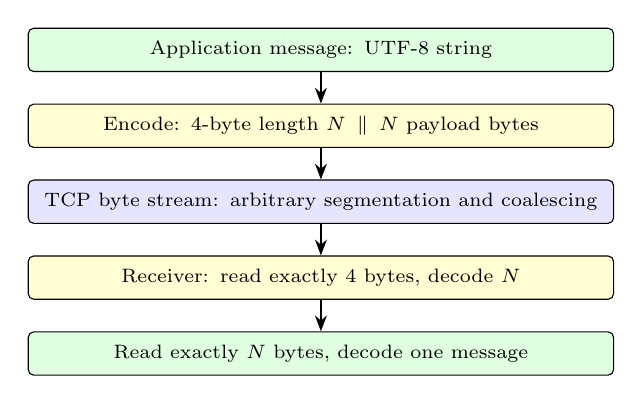
\begin{tikzpicture}[
  box/.style={draw, rounded corners=2pt, font=\scriptsize, minimum height=5.5mm, text width=7.2cm, align=center},
  arr/.style={-{Stealth[length=2mm]}, thick}
]
\node[box, fill=green!12] (a) {Application message: UTF-8 string};
\node[box, fill=yellow!18, below=4mm of a] (b) {Encode: 4-byte length $N$ \,$\Vert$\, $N$ payload bytes};
\node[box, fill=blue!10, below=4mm of b] (c) {TCP byte stream: arbitrary segmentation and coalescing};
\node[box, fill=yellow!18, below=4mm of c] (d) {Receiver: read exactly 4 bytes, decode $N$};
\node[box, fill=green!12, below=4mm of d] (e) {Read exactly $N$ bytes, decode one message};
\draw[arr] (a)--(b); \draw[arr] (b)--(c); \draw[arr] (c)--(d); \draw[arr] (d)--(e);
\end{tikzpicture}
\caption{Length-prefixed framing over a TCP byte stream.}
\label{fig:framing}
\end{figure}

\begin{lstlisting}[caption={Framing logic of the reference implementation (\texttt{protocol.py}, condensed).},label={lst:frame},float=t]
MAX_MESSAGE_BYTES = 4096

def send_message(conn, message):
    payload = message.encode("utf-8")
    if len(payload) > MAX_MESSAGE_BYTES:
        raise ValueError("message is too large")
    conn.sendall(struct.pack("!I", len(payload)) + payload)

def receive_message(conn):
    header = _receive_exactly(conn, 4)
    if header is None:
        return None            # peer closed
    (length,) = struct.unpack("!I", header)
    if length == 0 or length > MAX_MESSAGE_BYTES:
        raise ValueError("invalid message length")
    payload = _receive_exactly(conn, length)
    if payload is None:
        return None
    return payload.decode("utf-8")
\end{lstlisting}

\subsection{Concurrency Models for Servers}
A chat server holds many connections open for a long time, and most of the time each one is idle. Four models are usually contrasted. \emph{Thread-per-client} gives each connection a sequential control flow that is easy to read and debug, at the cost of one stack and one scheduling entity per client. A \emph{thread pool} bounds the number of workers but adds queueing and makes long-lived connections awkward. An \emph{event loop} multiplexes many connections on few threads using readiness notification, which scales further but forces the programmer to express each connection as a state machine \cite{kegel,krohn}. \emph{Staged} architectures split a service into event-driven stages joined by explicit queues with dynamic resource control \cite{seda}. The debate between threads and events is old and unresolved: Ousterhout argued that threads are the wrong abstraction for most purposes, von Behren \emph{et al.} argued that the objections are really objections to particular thread implementations, and Lee described the difficulty of reasoning about shared-memory threads \cite{ousterhout,vonbehren,lee}.

\subsection{Group Delivery and Topology}
Delivering one message to many recipients can be done in several ways. A central server can relay by repeated unicast, sending a separate copy on each connection. Peer-to-peer designs remove the relay but introduce membership, connection-count and consistency problems. IP multicast sends one datagram to a group, but it uses datagram semantics, which moves loss recovery, ordering and membership back to the application \cite{rfc1112}. Broker-based publish--subscribe decouples senders and receivers in space, time and synchronisation \cite{eugster}. Repeated unicast is not Ethernet broadcast or IP multicast: every recipient has an independent TCP connection with its own flow-control window and failure state.

\subsection{Security Considerations}
A trusted LAN reduces deployment effort but is not a security mechanism. On a plaintext channel, any reachable host can connect, choose any name, inject messages, and read traffic. TLS~1.3 protects a client--server channel against eavesdropping, tampering and forgery and can authenticate the server with a certificate \cite{rfc8446}. It does not authenticate individual users, and the server still sees plaintext after decryption. End-to-end secrecy between users needs a different construction, such as the Double Ratchet used by Signal, which provides forward secrecy and post-compromise security \cite{signal,cohngordon}. Unger \emph{et al.} give a systematic comparison of secure-messaging designs \cite{unger}.

%======================================================================
\section{Literature Review}
%======================================================================
Rather than reviewing sources one by one, it is more useful to group them by the design question they answer. Table~\ref{tab:comparison} compares the approaches discussed below, and the reference implementation, on the properties most relevant to a small LAN chat system.

\begin{table*}[t]
\centering
\caption{Comparative Analysis of Reviewed Approaches}
\label{tab:comparison}
\scriptsize
\renewcommand{\arraystretch}{1.1}
\begin{tabularx}{\textwidth}{@{}>{\raggedright\arraybackslash}p{2.6cm} Y Y Y Y Y Y@{}}
\toprule
\textbf{Approach} & \textbf{Transport} & \textbf{Framing} & \textbf{Topology} & \textbf{Security} & \textbf{Persistence} & \textbf{Key limitation for a small teaching system} \\
\midrule
IRC \cite{rfc1459,rfc2812} & TCP & CRLF lines, 512-byte limit & Server network & None in base spec & None & Text-only framing; limits fixed by the spec \\
XMPP \cite{rfc6120,rfc6121} & TCP & XML stream & Federated client--server & SASL and TLS & Via extensions & Heavy parser; large specification surface \\
MQTT 5.0 \cite{mqtt5} & TCP (optionally TLS) & Binary header, variable length & Broker pub/sub & Optional; credentials in CONNECT & Sessions and QoS & Needs a broker; more machinery than a chat room needs \\
WebSocket \cite{rfc6455} & TCP after HTTP upgrade & Length-carrying frames; client masking & Client--server & TLS via \code{wss} & None & Needs an HTTP handshake and a framework \\
Signal / Double Ratchet \cite{signal,cohngordon} & Any & Not specified & Relayed & End-to-end & Server-dependent & Cryptographic design, not a transport or server design \\
Flash \cite{flash} & TCP (web) & HTTP & Client--server & N/A & N/A & Web workload; compares process, thread and event models \\
SEDA \cite{seda} & TCP (services) & Application-defined & Staged pipeline & N/A & N/A & Targets far larger loads than a classroom chat \\
Threads vs.\ events \cite{ousterhout,vonbehren,krohn} & TCP & N/A & N/A & N/A & N/A & Position papers, not chat-specific \\
Reliable groups \cite{birman87,birman93} & Reliable channels & N/A & Process groups & N/A & Varies & Guarantees far beyond a demonstration system \\
\textbf{Reference implementation} & \textbf{TCP} & \textbf{4-byte length + UTF-8} & \textbf{Central relay} & \textbf{None} & \textbf{None} & \textbf{Trusted-LAN scope; hardened design proposed in Sec.~V} \\
\bottomrule
\end{tabularx}
\end{table*}

\textbf{Complete messaging protocols.} IRC was the first widely deployed text chat protocol on TCP. Its base specification frames messages as lines ending in carriage return and line feed, limited to 512 characters, and connects servers in a network so that users on different servers can talk to each other \cite{rfc1459,rfc2812}. The design is easy to implement by hand, which explains its longevity, but the delimiter approach forces every reader to agree on how to handle over-long or malformed lines. XMPP takes the opposite direction: it defines a long-lived XML stream over TCP with negotiation of TLS and SASL authentication, and a separate specification adds rosters and presence for instant messaging \cite{rfc6120,rfc6121}. That richness is precisely what makes it heavy for a small system. MQTT~5.0 places a broker between publishers and subscribers and adds quality-of-service levels, sessions and a compact binary header \cite{mqtt5}. WebSocket adds an HTTP-compatible opening handshake and then exchanges length-carrying frames, which makes it the natural route to browser clients \cite{rfc6455}. All four solve interoperability and deployment problems that a command-line demonstration deliberately sidesteps.

\textbf{Server-architecture research.} Pai, Druschel and Zwaenepoel compared multi-process, multi-threaded, single-process event-driven and asymmetric event-driven designs in the Flash web server and showed that architecture materially changes throughput and blocking behaviour \cite{flash}. SEDA proposed decomposing a service into stages linked by bounded queues, with dynamic controllers that keep the system stable under overload \cite{seda}. Position papers on both sides of the threads-versus-events debate followed \cite{ousterhout,vonbehren,lee}, and Krohn \emph{et al.} argued that event-driven code can be written with a structure close to threaded code \cite{krohn}. The C10K discussion collected the operating-system techniques needed to serve ten thousand simultaneous connections \cite{kegel}. What these works share is that their target workloads are much larger and more heterogeneous than a room of a few terminals. They justify an architectural boundary, meaning the point at which thread-per-client stops being adequate, without proving that threads are the wrong choice below it.

\textbf{Group communication and reliability.} Birman and Joseph's work on virtual synchrony and the later process-group approach show what \emph{reliable} group delivery means when processes can fail: members agree on group views and on the order in which messages are delivered relative to membership changes \cite{birman87,birman93}. Eugster \emph{et al.} survey publish--subscribe and classify it by how it decouples producers and consumers \cite{eugster}. A chat server that relays by repeated unicast provides none of these guarantees. A message accepted by the server can reach some clients before another connection fails, and there is no acknowledgement set, replay or globally stable order. Distinguishing this from transport reliability is important, because TCP's reliability is easily mistaken for delivery reliability.

\textbf{Secure messaging.} TLS~1.3 secures the channel \cite{rfc8446}, and the secure-messaging literature separates transport security, user authentication, authorisation, and end-to-end secrecy as distinct layers \cite{unger}. Signal's Double Ratchet shows how end-to-end secrecy with forward secrecy can be combined with an untrusted relay \cite{signal,cohngordon}. These layers are additive, and a system can adopt them in stages.

\textbf{Foundational texts.} Stevens' treatment of the sockets API and the standard networking textbooks remain the main sources for how a program actually uses TCP \cite{stevens,tanenbaum,kurose}.

Read together, these groups trace a fairly clean progression: from byte-stream transport, to explicit message framing, to concurrent servers, to full messaging protocols, and finally to reliable and secure group communication. What none of them does individually is present a compact, dependency-free system in which all of these decisions interact and can be inspected and measured at once.

%======================================================================
\section{Research Gap}
%======================================================================
Reading Table~\ref{tab:comparison} left to right, every reviewed approach is strong in the columns it was designed for and silent elsewhere. The remainder of this section explains why closing the gaps is a matter of design, not of adding one more feature.

\textbf{Framing, concurrency and shutdown are studied separately.} Protocol standards specify frames, architecture papers compare schedulers, and textbooks teach sockets and threads as independent exercises. In a real chat server they interact: a handler thread blocks inside a read while another thread wants to shut the server down, a broadcast iterates a client table while another handler removes an entry, and a half-received frame is abandoned when a peer disconnects mid-message. Few sources examine these interactions in a system small enough to read in one sitting.

\textbf{Sequential broadcast has a head-of-line risk.} When a handler sends a message to every recipient in turn, a slow receiver whose send buffer is full can delay delivery to every recipient after it. Per-client outbound queues with writer workers, bounded queues with a disconnect-or-drop policy, or non-blocking writes isolate slow consumers. This is well known in large systems \cite{seda}, but it is rarely shown in a teaching-scale implementation together with the code and tests that demonstrate the problem.

\textbf{Liveness detection is left to defaults.} Because TCP keep-alive is optional and off by default \cite{rfc1122}, a suspended laptop or an unplugged cable can leave a connection half-open for a long time. Explicit exit and exception cleanup cover normal termination, but abnormal termination needs a heartbeat or timeout that is seldom included in small examples.

\textbf{Security is either absent or arrives all at once.} Simple demonstrations are plaintext with no identity; production systems bring TLS, accounts and end-to-end encryption together \cite{rfc8446,unger,signal}. The intermediate steps, such as wrapping sockets with the standard \code{ssl} module and adding a name-uniqueness rule, are rarely presented as a staged path with a clear statement of what each stage does and does not protect.

\textbf{Evaluation is anecdotal.} Very few small messaging examples come with a protocol-correctness test that fragments and coalesces frames, or with a measurement method for latency and fan-out cost. Without one, no claim about when thread-per-client stops being adequate can be checked.

The reference design in Section~V is built around the premise that these gaps share one root cause: transport, framing, concurrency, delivery and security are presented as separate problems, when in a chat system they are stages of one path that must agree on message size limits, lifecycle and failure handling.

%======================================================================
\section{Reference Implementation and Proposed Hardened Design}
%======================================================================

\subsection{Reference Implementation}
The case-study system is a command-line chat program written with only the Python standard library \cite{pysocket,pythreading,pystruct}. It is split across five source files, mapped to networking concepts in Table~\ref{tab:mapping}. The statements below were verified against the source code.

\begin{figure}[t]
\centering
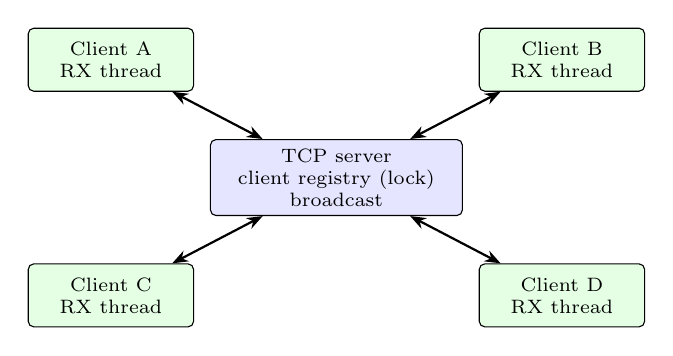
\begin{tikzpicture}[
  node distance=5mm,
  srv/.style={draw, rounded corners=2pt, fill=blue!10, font=\scriptsize, align=center, minimum width=3.2cm, minimum height=9mm},
  cli/.style={draw, rounded corners=2pt, fill=green!10, font=\scriptsize, align=center, minimum width=2.1cm, minimum height=8mm},
  arr/.style={{Stealth[length=2mm]}-{Stealth[length=2mm]}, thick}
]
\node[srv] (s) {TCP server \\ client registry (lock) \\ broadcast};
\node[cli, above left=6mm and 2mm of s] (a) {Client A \\ RX thread};
\node[cli, above right=6mm and 2mm of s] (b) {Client B \\ RX thread};
\node[cli, below left=6mm and 2mm of s] (c) {Client C \\ RX thread};
\node[cli, below right=6mm and 2mm of s] (d) {Client D \\ RX thread};
\draw[arr] (a)--(s); \draw[arr] (b)--(s); \draw[arr] (c)--(s); \draw[arr] (d)--(s);
\end{tikzpicture}
\caption{Centralised architecture of the reference implementation. Each client keeps one full-duplex TCP connection; the server owns membership and relays each message by repeated unicast, one handler thread per client.}
\label{fig:arch}
\end{figure}

\textbf{Server.} The server binds a TCP listening socket, runs an accept loop in a background thread, and starts one daemon thread per accepted connection. A handshake sends a \code{USERNAME} prompt and expects a name of one to 32 characters. Client state is held in a dictionary guarded by a \code{threading.Lock}; broadcast takes a snapshot of the recipients under the lock and then sends outside it, so a blocking send does not hold the lock. Messages are relayed to every client except the sender, and join and leave notices are broadcast in the same way. The server accepts a \code{quit}, \code{stop} or \code{exit} command typed into its own terminal; on that command, or on Ctrl+C, it sends a shutdown notice to each client, closes every connection, and then closes the listener.

\textbf{Client.} The client connects, completes the handshake, and starts a background receive thread so that incoming messages are displayed while the user is typing. The main thread reads terminal input and sends each line. The \code{/quit} and \code{/exit} commands, end-of-input and Ctrl+C all lead to a clean exit. A small helper module adds ANSI colours only when output is a terminal.

\textbf{Protocol and tests.} The framing in Listing~\ref{lst:frame} is shared by both programs, so there is a single definition. Frames are limited to 4096 bytes, zero-length and oversized frames are rejected, and a premature end of stream is reported as \code{None} rather than as an exception. The test suite has three tests: a round trip over a socket pair, the closed-connection case, and rejection of an oversized message.

\begin{table*}[t]
\centering
\caption{Implementation Mapping and Honest Scope}
\label{tab:mapping}
\footnotesize
\begin{tabularx}{\textwidth}{@{}l l Y Y@{}}
\toprule
\textbf{Component} & \textbf{Networking concept} & \textbf{Role in the system} & \textbf{Boundary / not provided} \\
\midrule
\code{server.py} & Listen, accept, membership, fan-out & Central relay; one daemon thread per client; lock-protected registry; graceful shutdown & Single server; no failover; sequential broadcast; no heartbeat \\
\code{client.py} & Active open; full-duplex I/O & Foreground input plus background receive thread; clean exit paths & No reconnect; no authenticated identity; no offline delivery \\
\code{protocol.py} & Record recovery over a stream & 4-byte network-order length; exact-read loop; 4096-byte limit; rejects zero-length frames & Not versioned; no message types or acknowledgements \\
\code{colors.py} & Presentation formatting & ANSI colours, disabled when not a terminal & Terminal-escape handling is not protocol security \\
\code{test\_chat.py} & Protocol verification & Round trip, closed connection, oversized message & Not a measurement of scalability or security \\
\bottomrule
\end{tabularx}
\end{table*}

\textbf{Limits.} Several limits follow directly from the design and are stated here so that the system's contribution is not overstated. Broadcast sends to recipients one after another with no per-client queue or timeout, so a stalled receiver can delay the ones that follow. Usernames are not required to be unique, and there is no authentication, so any host that can reach the port can join under any name. Traffic is plaintext. There is no heartbeat, so a half-open connection is found only when a send fails. There is no history, so a client that reconnects sees nothing that happened while it was away. Thread-per-client is appropriate for a classroom LAN but uses one thread per connection.

\subsection{Proposed Hardened Design}
We call the proposed design \emph{LANChat-H} (H for hardened). It keeps the five-file structure and the dependency-free constraint, and extends the system in the four stages shown in Fig.~\ref{fig:proposed}. Each stage is independent and testable, and each carries forward the limit and lifecycle decisions of the one before it. Table~\ref{tab:existing} summarises how the result compares with the approaches reviewed.

\textbf{Stage 1 -- Robustness of the existing path.} Add a bounded per-client outbound queue with a writer thread, so that a slow receiver is disconnected or has messages dropped by a stated policy instead of delaying others. Add a heartbeat message and a receive timeout so that half-open connections are detected. Require unique usernames at the handshake. Extend the tests to split the four-byte header across writes, combine many frames in one write, close mid-payload and disconnect during a broadcast.

\textbf{Stage 2 -- Protocol structure.} Replace bare strings with typed messages (chat, join, leave, system, ping) carried inside the same length-prefixed frame, and add a version byte. This makes the protocol extensible without changing the framing decision defended in Section~II.

\textbf{Stage 3 -- Channel security and identity.} Wrap both ends of the socket with the standard \code{ssl} module for TLS \cite{rfc8446,pyssl}, and add a per-user credential check and separate authorisation for administrative commands such as the server shutdown. This addresses eavesdropping, tampering and impersonation on the channel; it does not provide end-to-end secrecy, because the server still sees plaintext.

\textbf{Stage 4 -- Asynchronous variant.} Implement the same protocol with \code{asyncio} \cite{pyasyncio} and compare it with the threaded server under identical workloads, so that the point at which thread-per-client stops being adequate is measured rather than assumed. Persistent history with sequence numbers and acknowledgements can be studied as a further extension.

\begin{figure*}[t]
\centering
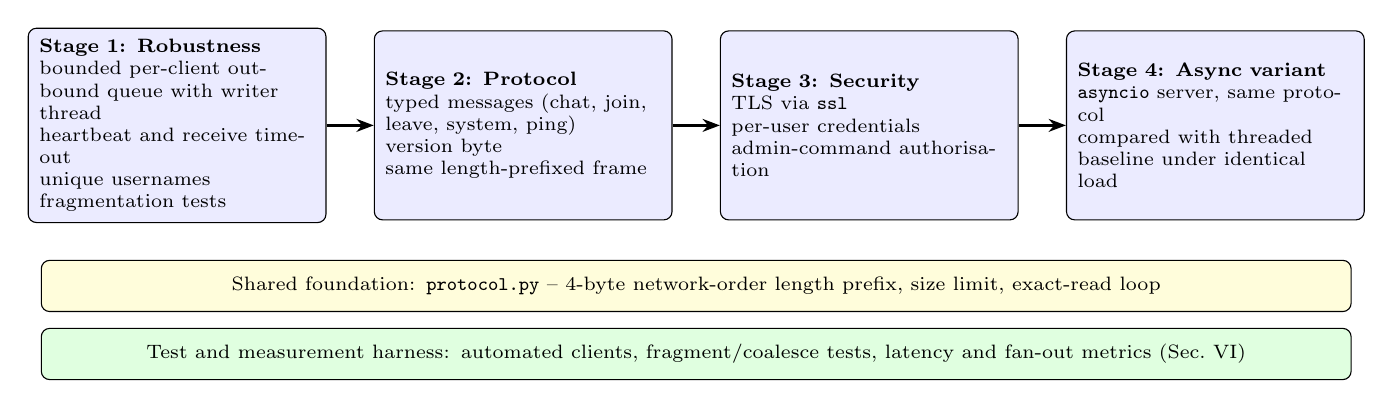
\begin{tikzpicture}[
  stage/.style={draw, rounded corners=3pt, fill=blue!8, font=\scriptsize, align=left, text width=3.5cm, minimum height=2.4cm, inner sep=4pt},
  bar/.style={draw, rounded corners=3pt, font=\scriptsize, align=center, minimum height=6.5mm, text width=16.4cm, anchor=north},
  arr/.style={-{Stealth[length=2.2mm]}, thick}
]
\node[stage] (s1) {\textbf{Stage 1: Robustness}\\ bounded per-client outbound queue with writer thread\\ heartbeat and receive timeout\\ unique usernames\\ fragmentation tests};
\node[stage, right=6mm of s1] (s2) {\textbf{Stage 2: Protocol}\\ typed messages (chat, join, leave, system, ping)\\ version byte\\ same length-prefixed frame};
\node[stage, right=6mm of s2] (s3) {\textbf{Stage 3: Security}\\ TLS via \texttt{ssl}\\ per-user credentials\\ admin-command authorisation};
\node[stage, right=6mm of s3] (s4) {\textbf{Stage 4: Async variant}\\ \texttt{asyncio} server, same protocol\\ compared with threaded baseline under identical load};
\draw[arr] (s1)--(s2); \draw[arr] (s2)--(s3); \draw[arr] (s3)--(s4);
\node[bar, fill=yellow!14] (f) at ($(s2.south east)+(3mm,-5mm)$) {Shared foundation: \texttt{protocol.py} -- 4-byte network-order length prefix, size limit, exact-read loop};
\node[bar, fill=green!12, below=2mm of f] (m) {Test and measurement harness: automated clients, fragment/coalesce tests, latency and fan-out metrics (Sec.~VI)};
\end{tikzpicture}
\caption{Overall architecture of the proposed LANChat-H design. Four independent stages extend the existing threaded server while sharing one framing definition and one test and measurement harness.}
\label{fig:proposed}
\end{figure*}

\begin{table}[t]
\centering
\caption{Existing Approaches vs.\ LANChat-H}
\label{tab:existing}
\footnotesize
\begin{tabularx}{\columnwidth}{@{}Y c c@{}}
\toprule
\textbf{Capability} & \textbf{Reviewed (individually)} & \textbf{LANChat-H} \\
\midrule
Explicit message framing & Yes & Yes \\
Frame-size limit enforced & Varies & Yes \\
Isolation of slow receivers & Large systems only & Yes \\
Liveness detection & Rare in small systems & Yes \\
Channel security (TLS) & Production systems & Yes (Stage 3) \\
Threaded and async comparison & No & Yes (Stage 4) \\
Frame-fragmentation tests & Rare & Yes \\
Single dependency-free artifact & No & Yes \\
\bottomrule
\end{tabularx}
\end{table}

%======================================================================
\section{Evaluation Plan}
%======================================================================
No valid performance conclusion can be drawn without measurements on a specified machine, Python version, LAN, payload distribution and client count, so none is reported here. A reproducible experiment should vary the number of clients $C$, the payload size $S$ and the offered message rate $R$. For a sender timestamp $t_s$ and a recipient timestamp $t_{r,i}$, the latency seen by recipient $i$ is
\begin{equation}
L_i = t_{r,i} - t_s .
\end{equation}
A broadcast is summarised by the median, 95th percentile and maximum of $L_i$, and by the completion spread
\begin{equation}
\Delta = \max_i L_i - \min_i L_i .
\end{equation}
Application throughput is the number of fully reconstructed frames per second, not raw TCP segments.

\textbf{Fan-out cost model.} The head-of-line risk described in Section~IV can be stated precisely. Let the server relay a message to $N$ recipients in a fixed order, and let $s_j$ be the time the blocking send to recipient $j$ takes. With sequential sends, recipient $k$ receives the message after
\begin{equation}
D_k = \sum_{j=1}^{k} s_j , \qquad T_{\text{bcast}} = D_N .
\end{equation}
If recipient $m$ stalls for an extra time $W$ because its send buffer is full, every later recipient is delayed by at least the same amount:
\begin{equation}
D_k \;\ge\; W + \sum_{j=1}^{k} s_j \qquad \text{for all } k \ge m .
\end{equation}
With a bounded per-client queue and a writer thread (Stage 1), the server's send to each recipient reduces to an enqueue with cost $q_j \ll W$, so $D_k$ no longer depends on $W$ for $k \neq m$. Table~\ref{tab:metrics} lists the planned measurements; $D_k$ is measured directly, with and without an artificially slowed receiver, to confirm the effect.

\begin{table}[t]
\centering
\caption{Suggested Measurements}
\label{tab:metrics}
\footnotesize
\begin{tabularx}{\columnwidth}{@{}l Y Y@{}}
\toprule
\textbf{Metric} & \textbf{Method} & \textbf{Purpose} \\
\midrule
Latency & Monotonic timestamps at sender and receivers & End-to-end responsiveness \\
Throughput & Frames and bytes per second & Capacity under load \\
Fan-out cost & Delivery time vs.\ number of recipients & Broadcast scaling \\
CPU / memory & Process sampling under steady load & Thread and queue overhead \\
Failure recovery & Time from disconnect to cleanup notice & Fault responsiveness \\
Correctness & Fragmented and coalesced frames in tests & Verify exact-read framing \\
\bottomrule
\end{tabularx}
\end{table}

The harness should generate automated clients, start trials together, warm the system up, run repeated fixed-duration trials, and report dispersion rather than a single best run. Adversarial cases should split the four-byte header across writes, combine many frames in one write, close in the middle of a payload, send zero-length and oversized frames, and disconnect during a broadcast, so that protocol correctness is evaluated separately from speed.

%======================================================================
\section{Conclusion}
%======================================================================
Taken together, the literature on TCP-based messaging tells a story of solid but scattered progress. Transport standards define a reliable byte stream, framing conventions recover messages from it, server-architecture research explains when threads give way to events, messaging protocols fix particular design points, and group-communication and security work describe guarantees well beyond a demonstration system. What this survey's comparison and gap analysis both point to is that no single small artifact walks through all of these decisions together in a form that can be read, tested and measured.

The four-byte length prefix with exact-read logic is a sound choice for a stream of UTF-8 text, thread-per-client is understandable and sufficient at classroom scale, and a central relay simplifies membership while creating a single point of failure. The reference implementation makes these choices explicitly and states what it omits. The hardened design proposed here carries the same limit and lifecycle decisions through bounded queues, heartbeats, typed messages, TLS and an asynchronous variant, so that each stage can be verified before the next is added. The next phase is to implement the four stages, run the measurement plan of Section~VI on a specified LAN, and report the results, including where the threaded design stops being adequate.

%======================================================================
\balance
\begin{thebibliography}{99}
\bibitem{rfc793} J. Postel, ``Transmission Control Protocol,'' IETF, RFC 793, Sep. 1981.
\bibitem{rfc9293} W. Eddy, Ed., ``Transmission Control Protocol (TCP),'' IETF, RFC 9293, Aug. 2022.
\bibitem{rfc1122} R. Braden, Ed., ``Requirements for Internet Hosts -- Communication Layers,'' IETF, RFC 1122, Oct. 1989.
\bibitem{jacobson} V. Jacobson, ``Congestion avoidance and control,'' in \emph{Proc. ACM SIGCOMM}, 1988, pp. 314--329.
\bibitem{rfc5681} M. Allman, V. Paxson, and E. Blanton, ``TCP congestion control,'' IETF, RFC 5681, Sep. 2009.
\bibitem{saltzer} J. H. Saltzer, D. P. Reed, and D. D. Clark, ``End-to-end arguments in system design,'' \emph{ACM Trans. Comput. Syst.}, vol. 2, no. 4, pp. 277--288, 1984.
\bibitem{stevens} W. R. Stevens, B. Fenner, and A. M. Rudoff, \emph{UNIX Network Programming, Vol. 1: The Sockets Networking API}, 3rd ed. Addison-Wesley, 2003.
\bibitem{tanenbaum} A. S. Tanenbaum and D. J. Wetherall, \emph{Computer Networks}, 5th ed. Pearson, 2011.
\bibitem{kurose} J. F. Kurose and K. W. Ross, \emph{Computer Networking: A Top-Down Approach}, 8th ed. Pearson, 2021.
\bibitem{rfc3629} F. Yergeau, ``UTF-8, a transformation format of ISO 10646,'' IETF, RFC 3629, Nov. 2003.
\bibitem{flash} V. S. Pai, P. Druschel, and W. Zwaenepoel, ``Flash: An efficient and portable Web server,'' in \emph{Proc. USENIX Annu. Tech. Conf.}, 1999.
\bibitem{seda} M. Welsh, D. Culler, and E. Brewer, ``SEDA: An architecture for well-conditioned, scalable Internet services,'' in \emph{Proc. ACM SOSP}, 2001, pp. 230--243.
\bibitem{ousterhout} J. K. Ousterhout, ``Why threads are a bad idea (for most purposes),'' invited talk, USENIX Winter Tech. Conf., 1996.
\bibitem{vonbehren} R. von Behren, J. Condit, and E. Brewer, ``Why events are a bad idea (for high-concurrency servers),'' in \emph{Proc. HotOS IX}, 2003.
\bibitem{lee} E. A. Lee, ``The problem with threads,'' \emph{Computer}, vol. 39, no. 5, pp. 33--42, May 2006.
\bibitem{krohn} M. Krohn, E. Kohler, and M. F. Kaashoek, ``Events can make sense,'' in \emph{Proc. USENIX Annu. Tech. Conf.}, 2007.
\bibitem{kegel} D. Kegel, ``The C10K problem,'' 1999. [Online]. Available: http://www.kegel.com/c10k.html
\bibitem{rfc1459} J. Oikarinen and D. Reed, ``Internet Relay Chat protocol,'' IETF, RFC 1459, May 1993.
\bibitem{rfc2812} C. Kalt, ``Internet Relay Chat: Client protocol,'' IETF, RFC 2812, Apr. 2000.
\bibitem{rfc6120} P. Saint-Andre, ``Extensible Messaging and Presence Protocol (XMPP): Core,'' IETF, RFC 6120, Mar. 2011.
\bibitem{rfc6121} P. Saint-Andre, ``Extensible Messaging and Presence Protocol (XMPP): Instant messaging and presence,'' IETF, RFC 6121, Mar. 2011.
\bibitem{rfc6455} I. Fette and A. Melnikov, ``The WebSocket protocol,'' IETF, RFC 6455, Dec. 2011.
\bibitem{mqtt5} OASIS, ``MQTT Version 5.0,'' OASIS Standard, Mar. 2019.
\bibitem{rfc1112} S. Deering, ``Host extensions for IP multicasting,'' IETF, RFC 1112, Aug. 1989.
\bibitem{eugster} P. Th. Eugster, P. A. Felber, R. Guerraoui, and A.-M. Kermarrec, ``The many faces of publish/subscribe,'' \emph{ACM Comput. Surv.}, vol. 35, no. 2, pp. 114--131, Jun. 2003.
\bibitem{birman87} K. P. Birman and T. A. Joseph, ``Reliable communication in the presence of failures,'' \emph{ACM Trans. Comput. Syst.}, vol. 5, no. 1, pp. 47--76, 1987.
\bibitem{birman93} K. P. Birman, ``The process group approach to reliable distributed computing,'' \emph{Commun. ACM}, vol. 36, no. 12, pp. 37--53, Dec. 1993.
\bibitem{rfc8446} E. Rescorla, ``The Transport Layer Security (TLS) protocol version 1.3,'' IETF, RFC 8446, Aug. 2018.
\bibitem{unger} N. Unger \emph{et al.}, ``SoK: Secure messaging,'' in \emph{Proc. IEEE Symp. Security and Privacy}, 2015, pp. 232--249.
\bibitem{cohngordon} K. Cohn-Gordon, C. Cremers, B. Dowling, L. Garratt, and D. Stebila, ``A formal security analysis of the Signal messaging protocol,'' in \emph{Proc. IEEE Eur. Symp. Security and Privacy}, 2017, pp. 451--466.
\bibitem{signal} M. Marlinspike and T. Perrin, ``The Double Ratchet algorithm,'' Signal, Rev. 1, Nov. 2016.
\bibitem{pysocket} Python Software Foundation, ``socket,'' \emph{Python 3 Documentation}. \url{https://docs.python.org/3/library/socket.html}
\bibitem{pythreading} Python Software Foundation, ``threading,'' \emph{Python 3 Documentation}. \url{https://docs.python.org/3/library/threading.html}
\bibitem{pystruct} Python Software Foundation, ``struct,'' \emph{Python 3 Documentation}. \url{https://docs.python.org/3/library/struct.html}
\bibitem{pyssl} Python Software Foundation, ``ssl,'' \emph{Python 3 Documentation}. \url{https://docs.python.org/3/library/ssl.html}
\bibitem{pyasyncio} Python Software Foundation, ``asyncio,'' \emph{Python 3 Documentation}. \url{https://docs.python.org/3/library/asyncio.html}
\end{thebibliography}

\end{document}
